\documentclass[tikz,border=6pt]{standalone}

    \usepackage{tikz}
    % file/folder tree
    \usepackage[edges]{forest}
    \newlength\Size
    \usepackage{amsmath}
    %    \usepackage{verbatim}
    \usepackage{fontspec}
    \setmainfont{Arial}

\begin{document}


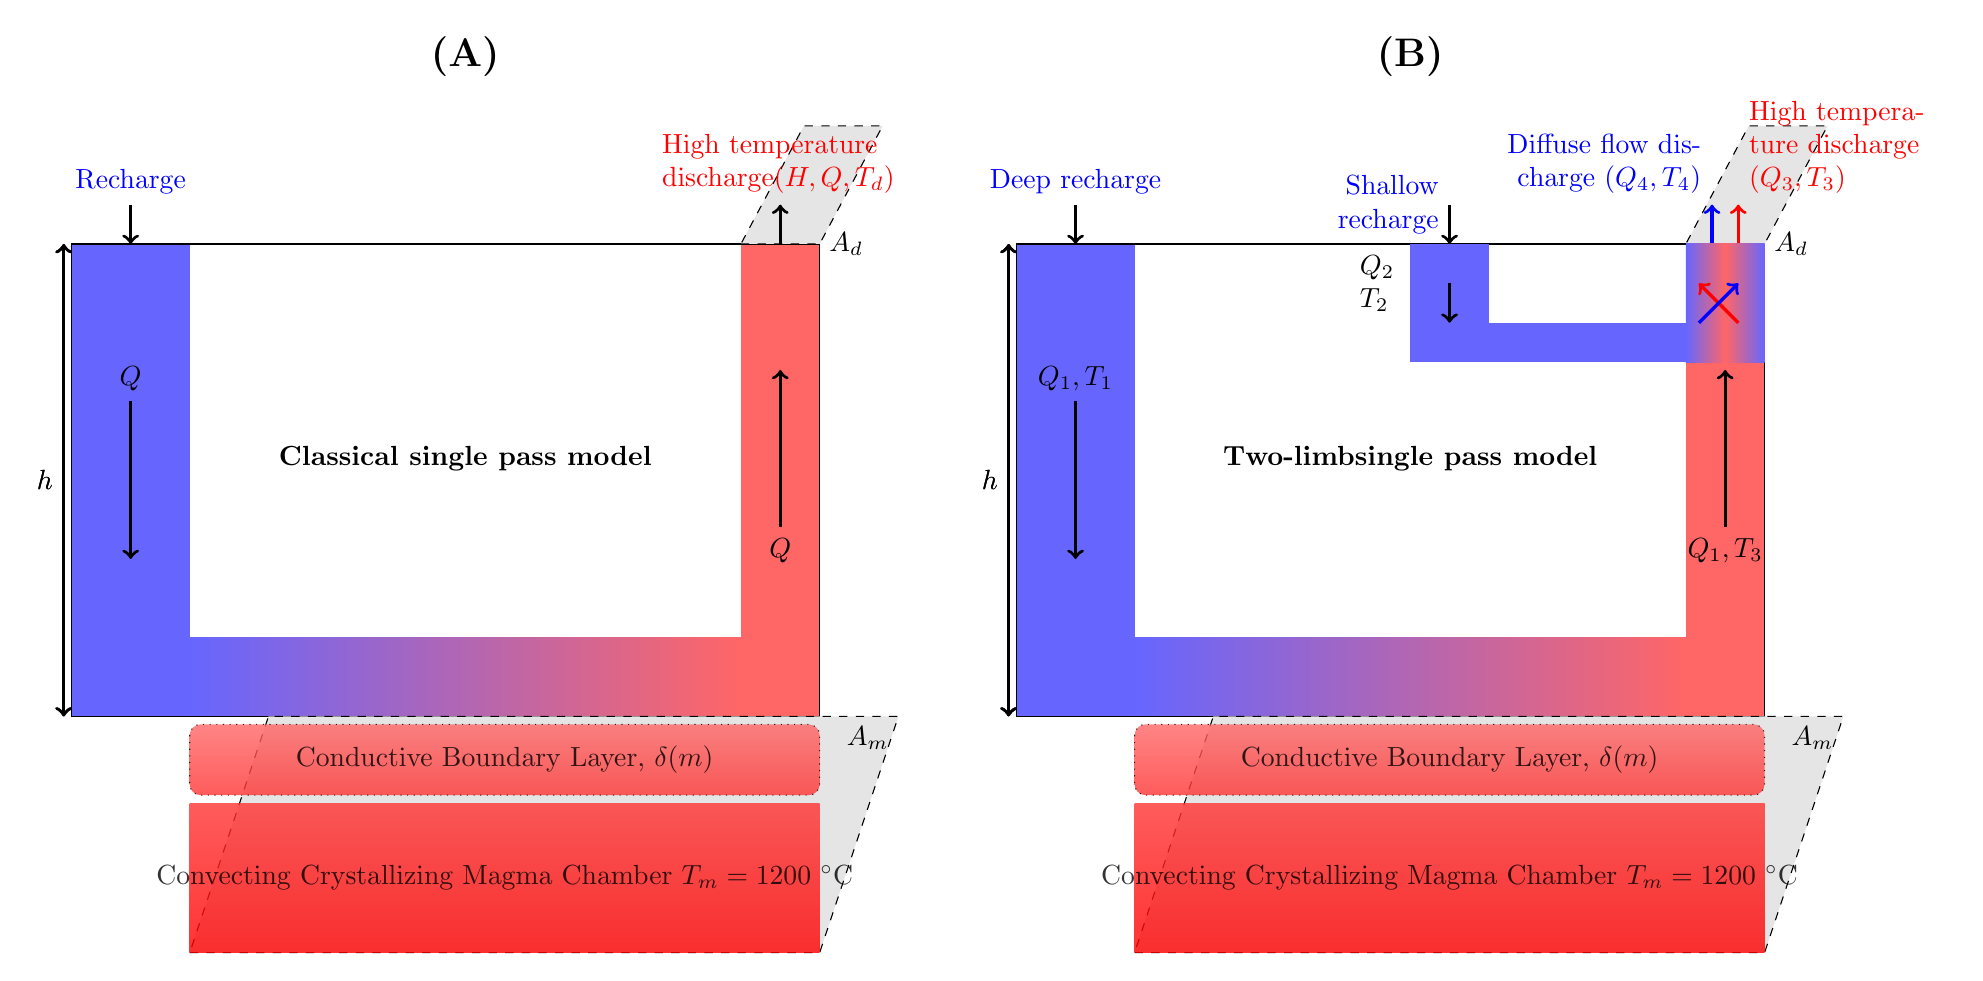
\begin{tikzpicture}
    \def\x0{0.5}
    \def\y0{1}
    \def\hmodel{6}
    \def\wmodel{7}
    \def\wleft{1.5}
    \def\thickbottom{1}
    \def\wright{1}
    \def\cleft{blue!60}
    \def\cright{red!60}
    
    %\draw [help lines] (0,0) grid (14,8);
    %	left branch: recharge zone
    \path[draw=none, fill=\cleft] (\x0,\y0) rectangle (\x0+\wleft,\y0+\hmodel);
    %	bottom: 
    \shade [left color=\cleft,right color=\cright](\x0+\wleft,\y0) rectangle (\x0+\wleft+\wmodel,\y0+\thickbottom);
    %	right branch: discharge zone
    \path[draw=none, fill=\cright] (\x0+\wleft+\wmodel,\y0) rectangle (\x0+\wleft+\wmodel+\wright,\y0+\hmodel);
    %	boundary
    \path[draw=black, fill=none] (\x0,\y0) rectangle (\x0+\wleft+\wright+\wmodel,\y0+\hmodel);
    %	bottom: 
    \path [draw=black,dashed,fill=gray!20] (\x0+\wleft,\y0-\thickbottom-\thickbottom-\thickbottom) -- +(\wmodel+\wright,0) -- +(\wmodel+\wright+1,3) node[below left] {$A_m$} -- +(1,3) -- cycle;
    \shade [bottom color=red!80,top color=\cright,opacity=0.8,rounded corners,draw=black,dotted](\x0+\wleft,\y0-0.1) rectangle (\x0+\wleft+\wmodel+\wright,\y0-\thickbottom) node[pos=0.5]{Conductive Boundary Layer, $\delta(m)$};
    
    \shade [bottom color=red,top color=red!80,opacity=0.8](\x0+\wleft,\y0-\thickbottom-0.1) rectangle (\x0+\wleft+\wmodel+\wright,\y0-\thickbottom-\thickbottom-\thickbottom) node[pos=0.5] {Convecting Crystallizing \linebreak Magma Chamber $T_m = 1200 \ ^{\circ}$C };
    
    %标注
    %recharge
    \draw[->,very thick] (\x0+\wleft/2,\y0+4) node[above] {$Q$} -- +(0,-2);
    \draw[<->,very thick] (\x0-0.1,\y0) -- (\x0-0.1,\y0+\hmodel) node[pos=.5,left]  {$h$} ;
    \draw[->,very thick] (\x0+\wleft/2,\y0+\hmodel+0.5) node[above] {\textcolor{blue}{Recharge}} -- +(0,-0.5);
    %discharge
    \draw[<-,very thick] (\x0+\wmodel+\wleft+\wright/2,\y0+4.4)  -- +(0,-2) node[below] {$Q$};
    \draw[<->,very thick] (\x0-0.1,\y0) -- (\x0-0.1,\y0+\hmodel) node[pos=.5,left]  {$h$} ;
    \path [draw=black,dashed, fill=gray!20] (\x0+\wleft+\wmodel,\y0+\hmodel) -- +(\wright,0) node[ right] {$A_{d}$} -- +(\wright+0.8,1.5) -- +(0.8,1.5) -- cycle;
    
    \draw[<-,very thick] (\x0+\wleft+\wmodel+0.5,\y0+\hmodel+0.5) node[above, text width=3cm] {\textcolor{red}{High temperature discharge($H, Q, T_d$)}} -- +(0,-0.5);
    \node[above](a) at (\x0+\wleft+\wmodel/2, \y0+\hmodel+2){\Large{\textbf{(A)}}};
    \node[above](a) at (\x0+\wleft+\wmodel/2, \y0+\hmodel/2){{\textbf{Classical single pass model}}};
    
%    two-limb single pass model
\def\x0{12.5}
\def\y0{1}
%	left branch: recharge zone
\path[draw=none, fill=\cleft] (\x0,\y0) rectangle (\x0+\wleft,\y0+\hmodel);
%	bottom: 
\shade [left color=\cleft,right color=\cright](\x0+\wleft,\y0) rectangle (\x0+\wleft+\wmodel,\y0+\thickbottom);
%	right branch: discharge zone
\path[draw=none, fill=\cright] (\x0+\wleft+\wmodel,\y0) rectangle (\x0+\wleft+\wmodel+\wright,\y0+\hmodel);
%	boundary
\path[draw=black, fill=none] (\x0,\y0) rectangle (\x0+\wleft+\wright+\wmodel,\y0+\hmodel);
%	bottom: 
\path [draw=black,dashed,fill=gray!20] (\x0+\wleft,\y0-\thickbottom-\thickbottom-\thickbottom) -- +(\wmodel+\wright,0) -- +(\wmodel+\wright+1,3) node[below left] {$A_m$} -- +(1,3) -- cycle;
\shade [bottom color=red!80,top color=\cright,opacity=0.8,rounded corners,draw=black,dotted](\x0+\wleft,\y0-0.1) rectangle (\x0+\wleft+\wmodel+\wright,\y0-\thickbottom) node[pos=0.5]{Conductive Boundary Layer, $\delta(m)$};

\shade [bottom color=red,top color=red!80,opacity=0.8](\x0+\wleft,\y0-\thickbottom-0.1) rectangle (\x0+\wleft+\wmodel+\wright,\y0-\thickbottom-\thickbottom-\thickbottom) node[pos=0.5] {Convecting Crystallizing \linebreak Magma Chamber $T_m = 1200 \ ^{\circ}$C };
%标注
%recharge
\draw[->,very thick] (\x0+\wleft/2,\y0+4) node[above] {$Q_1, T_1$} -- +(0,-2);
%\draw[] (\x0+1,\y0+5) node[above,text width=1cm] {$T_1$} -- (\x0+1,3);
\draw[<->,very thick] (\x0-0.1,\y0) -- (\x0-0.1,\y0+\hmodel) node[pos=.5,left]  {$h$} ;
\draw[->,very thick] (\x0+\wleft/2,\y0+\hmodel+0.5) node[above] {\textcolor{blue}{Deep recharge}} -- +(0,-0.5);
%discharge
\draw[<-,very thick] (\x0+\wmodel+\wleft+\wright/2,\y0+4.4)  -- +(0,-2) node[below] {$Q_1, T_3$};
\draw[<->,very thick] (\x0-0.1,\y0) -- (\x0-0.1,\y0+\hmodel) node[pos=.5,left]  {$h$} ;
\path [draw=black,dashed, fill=gray!20] (\x0+\wleft+\wmodel,\y0+\hmodel) -- +(\wright,0) node[ right] {$A_{d}$} -- +(\wright+0.8,1.5) -- +(0.8,1.5) -- cycle;

\draw[->,very thick, color=red] (\x0+\wleft+\wmodel+\wright/3*2,\y0+\hmodel)  -- +(0,0.5) node[above right, text width=2.5cm] {\textcolor{red}{High temperature discharge ($Q_3, T_3$)}};
\draw[->,very thick, color=blue] (\x0+\wleft+\wmodel+\wright/3,\y0+\hmodel)  -- +(0,0.5) node[above left, text width=2.5cm, align=right] {\textcolor{blue}{Diffuse flow discharge ($Q_4, T_4$)}};
\node[above](a) at (\x0+\wleft+\wmodel/2, \y0+\hmodel+2){\Large{\textbf{(B)}}};
    \node[above](a) at (\x0+\wleft+\wmodel/2, \y0+\hmodel/2){{\textbf{Two-limbsingle pass model}}};
    
%the second limb
\def\x0{17.5}
\def\y0{5.5}
\def\hmodel{1.5}
\def\wmodel{2.5}
\def\wleft{1}
\def\thickbottom{0.5}
\def\wright{1}
\def\cleft{blue!60}
\def\cright{red!60}
%	left branch: recharge zone
\path[draw=none, fill=\cleft] (\x0,\y0) rectangle (\x0+\wleft,\y0+\hmodel);
%	bottom: 
\path [draw=none, fill=\cleft](\x0+\wleft,\y0) rectangle (\x0+\wleft+\wmodel,\y0+\thickbottom);
%	right branch: discharge zone
\shade [left color=\cleft,right color=\cright] (\x0+\wleft+\wmodel,\y0) rectangle (\x0+\wleft+\wmodel+\wright/2,\y0+\hmodel);
\shade [left color=\cright,right color=\cleft] (\x0+\wleft+\wmodel+\wright/2,\y0) rectangle (\x0+\wleft+\wmodel+\wright,\y0+\hmodel);

\draw[->,very thick, color=red] (\x0+\wleft+\wmodel+\wright/3*2,\y0+\hmodel-1)  -- +(-\wright/2,0.5) ;
\draw[<-,very thick, color=blue] (\x0+\wleft+\wmodel+\wright/3*2,\y0+\hmodel-0.5)  -- +(-\wright/2,-0.5) ;
\draw[<-,very thick] (\x0+\wleft/2,\y0+\hmodel) -- +(0,0.5) node[left, text width=2cm, align=right] {\textcolor{blue}{Shallow recharge}} ;

\draw[<-,very thick] (\x0+\wleft/2,\y0+\hmodel-1) -- +(0,0.5) node[left, text width=1cm, align=left] {$Q_2$ \ $T_2$} ;

\end{tikzpicture}
    
\end{document}


